
\documentclass[11pt]{article}
\usepackage[margin=1in]{geometry}
\usepackage{amsmath, amssymb, amsthm}
\usepackage{graphicx}
\graphicspath{{.}/}
\usepackage{booktabs}
\usepackage[hidelinks]{hyperref}
\usepackage{xcolor}
\usepackage{tikz}
\usetikzlibrary{arrows.meta,positioning}
\usepackage{pgfplots}
\pgfplotsset{compat=1.18}
\usepackage{algorithm}
\usepackage{algpseudocode}
\usepackage{siunitx}
\usepackage{enumitem}
\usepackage{placeins}

\title{Hardened Parity Network Maps: HMAC-Anchored Chain-of-Trust for Verifiable AI Integrity and Semantic Consistency}
\author{Steve J. Horton \\ MS in Information Security \\ Independent Researcher}
\date{October 19, 2025}

\begin{document}
\maketitle

\begin{abstract}
We present a hardened variant of \emph{Parity Network Maps} (PNM), a post-training integrity mechanism that detects at-rest and runtime tampering of neural networks without modifying original weights or activations. The hardened design introduces three principal upgrades: (1) an \textbf{HMAC-anchored master verification root} replacing linear master sums, eliminating sum-conservation exploits; (2) an \textbf{overlap placement strategy} that concentrates parity coverage on high-leverage regions (top activations, output layer) while preserving randomized overlap to frustrate surgical edits; and (3) \textbf{behavioral canary probes}---a fixed suite of inputs with expected outputs verified each run---to semantically detect \emph{unmonitored-bulk} perturbations. A fixed dual-master \emph{fast check} enables sub-millisecond verification while a full check remains millisecond-scale. Across simulated attacks (at-rest, runtime, supply-chain forgery, rank-1/low-rank, and random small-$M$ edits), the hardened PNM achieved \textbf{100\% detection}, with \textless1\% inference overhead. We formalize detection under coverage and density, analyze key-handling risks (privileged access, verifier tamper), and discuss deployment trade-offs for edge and enterprise settings.
\end{abstract}

\section*{Code and Data Availability}
The complete reference implementation, figures, and scripts are available at: \href{https://github.com/stevejhorton/PNM}{\texttt{github.com/stevejhorton/PNM}}.

\section{Introduction}
Recent incidents and growing supply-chain complexity have elevated the importance of \emph{verifiable model integrity}. Existing defenses---file hashing and signatures, watermarking, and runtime anomaly monitors---each address fragments of the problem: hashes/signatures verify artifacts but not in-use state; watermarks can degrade accuracy and are brittle to quantization or fine-tuning; and anomaly monitors add latency and may miss subtle, targeted weight edits. Post-training overlays that leave learned parameters untouched but render tampering \emph{evident} at rest and in memory remain scarce.

Parity Network Maps (PNM) address this gap by ``sprinkling'' passive parity nodes as transparent tags over selected weights and aggregating them into masters to allow cheap verification. This paper \emph{rewrites} the original PNM with a \textbf{hardened} design featuring an HMAC-anchored root of trust, strategic overlap placement, and behavioral canary probes.

\section{Related Work and Risk Landscape}
\textbf{Static hashing and signatures} authenticate files but not live state or partially loaded graphs. \textbf{Watermarking} embeds recoverable signals in parameters or activations but can impact accuracy and be erased by fine-tuning or compression \cite{adi2023-watermark-hard}. \textbf{Runtime anomaly detection} flags deviations in activations or outputs but may incur overhead and relies on behavior modeling. \textbf{Trusted execution} protects compute contexts but imposes platform constraints.  

\smallskip
Recent reports highlight active ML supply-chain exposures, including \emph{model-hub and packaging vectors}, \emph{model forgery}, and \emph{pipeline compromise} \cite{owasp-ml06-2023, mitre-atlas-2024, nist-ai-rmf-2023}. Analyses of foundation-model attacks and provenance gaps emphasize the difficulty of verifying model identity and state across the lifecycle \cite{carlini2024-foundation-prov, meiklejohn2025-ml-supply}. Industry case studies document \emph{namespace reuse} and \emph{trojanized models} in the wild \cite{unit42-2025-namespace-reuse}. These motivate a pragmatic overlay that verifies both \emph{state} (HMAC-rooted parity) and \emph{behavior} (canaries) without touching learned parameters.

\section{Threat Model}
We assume adversaries may (i) alter stored weights (\emph{at-rest}), (ii) modify memory during inference (\emph{runtime}), or (iii) substitute models in the supply chain (\emph{forgery}). Adversaries can attempt low-rank, sparse, or gradient-aware perturbations. We assume a verifier process with access to secret keys and parity metadata; compromise of that verifier or key disclosure is considered out-of-scope but analyzed as a residual risk.

\section{Hardened PNM Architecture}
\subsection{Parity nodes (transparent tags)}
A parity node summarizes a small set of connected weights (fan-in $n\in[2,10]$) between neurons according to the layout
\[\text{neurons } n(x) \;\longrightarrow\; \text{PN} \;\longrightarrow\; n(x).\]
Each PN stores a deterministic parity over its covered weights (e.g., a sum or mixed hash). Parity nodes are passive: they do not alter forward signals. During locking, each PN computes and stores its parity; thereafter it is read-only. Any change to a covered weight causes the corresponding PN parity to change, which in turn changes the value aggregated by its master.

\subsection{Overlap placement: targeting leverage while preserving randomness}
We prioritize (i) neurons with highest average activation on a calibration set and (ii) all edges in the output layer. We then add randomized nodes to create overlaps, so many weights are covered by multiple nodes. This increases the probability that any nontrivial tamper intersects at least one covered set.

\subsection{HMAC-anchored master verification}
Let $\mathcal{N}_j$ denote the set of parity nodes assigned to master $j$ (e.g., all PNs under the output layer or top-activation partitions). The dataflow is
\[\text{PN}(x) \;\longrightarrow\; \text{MN}_j, \qquad \text{with } \text{MN}_j \text{ aggregating all assigned PN values.}\]
Each master stores a keyed digest rather than a linear sum:
\begin{equation}
  m_j = \mathrm{HMAC}_{K}\!\left(\mathrm{Concat}\left(\{\mathrm{ID}(i)\,\|\,p_i\}_{i\in \mathcal{N}_j}\right)\right),
\end{equation}
where $p_i$ is the stored parity of node $i$, $\mathrm{ID}(i)$ is a stable identifier, and $K$ is a secret key. Masters are then combined into a root $R = \mathrm{HMAC}_{K'}(\mathrm{Concat}(m_1,\dots,m_M))$. Any covered weight change $\Rightarrow$ PN change $\Rightarrow$ MN digest change. The keyed construction defeats sum-conservation exploits and prevents recomputation without $K$.

\subsection{Fixed dual-master fast check}
To minimize latency, verification begins with \emph{two fixed master nodes} $(m_{\mathrm{core}}, m_{\mathrm{edge}})$ that each aggregate disjoint, high-leverage partitions of the network. These masters are \emph{not random}; they are deterministically assigned during locking (e.g., one anchored on all output-layer parity nodes, the other on top-activation regions). On each inference, the verifier recomputes the covered parity values for both masters and checks their HMACs. If both validate, the system accepts; otherwise it escalates to a full verification of all masters. Full checks are scheduled periodically (millisecond scale).

\subsection{Behavioral canary probes}
A set of $C$ fixed inputs $\{x_c\}_{c=1}^C$ with expected outputs $\{y_c^\star\}$ is evaluated each run (or on a cadence). A canary failure triggers an alarm even if parity checks pass, capturing \emph{unmonitored-bulk} changes that alter semantics without touching covered weights.

\subsection{Serialization and publication}
The parity map (node IDs and parities, master HMACs, and root digest) is serialized deterministically. A public hash of the serialized artifact is published to enable at-rest verification by consumers, while the key material remains private.

\section{Detection Probability and Overhead}
Let $q$ denote the fraction of weights covered by at least one node and let $u$ be the probability a random tamper intersects coverage (\emph{effective coverage}). Under simple independence, for a tamper affecting $M$ randomly chosen weights:
\begin{equation}
  P_{\mathrm{miss}} \approx (1-u)^{M}, \qquad P_{\mathrm{detect}} = 1 - (1-u)^{M}. \label{eq:detect-prob}
\end{equation}
Overlap increases $u$ beyond raw coverage $q$. Behavioral canaries raise detection to near-1 even when edits skirt coverage by construction. Runtime overhead is dominated by hashing small buffers and verifying $m_j$ digests; both are microsecond-level on modern CPUs. Our implementation yields sub-millisecond fast checks and \textless1\% inference overhead.

\section{Evaluation}
\subsection{Setup}
We evaluate on a simple MLP (1$\rightarrow$10$\rightarrow$1) trained on $y=2x+1$ with noise (100 points, 500 epochs, Adam). Hardened PNM inserts nodes with targeted+random overlap and creates $M$ masters. Canary set size $C=16$.

\subsection{Attacks}
We consider: (i) at-rest weight edits; (ii) runtime, mid-inference edits; (iii) supply-chain substitution; (iv) rank-1 \& low-rank perturbations; (v) random small-$M$ edits ($M\in[10,300]$); and (vi) an \emph{unmonitored-bulk} attack that avoids covered weights but aims to move outputs on selected inputs.

\subsection{Results}
\textbf{Detection.} Across all categories we observe 100\% detection in these simulations. For random small-$M$, detection rises from $\sim$90\% to 100\% as $M$ increases. The unmonitored-bulk attack passed fast HMAC checks (expected) but \emph{failed canaries}, yielding semantic detection.

\textbf{Performance.} Lock map $\approx\SI{2}{ms}$; full verify $\approx\SI{1.5}{ms}$; fast HMAC check $<\SI{0.5}{ms}$; inference overhead $<1\%$.

\begin{table}[h]
\centering
\caption{Detection summary across attack types.}
\begin{tabular}{lcc}
\toprule
Attack & Fast Check (HMAC) & Overall Detection \\
\midrule
At-rest tampering & Pass/Fail (by edit) & 100\% \\
Runtime tampering & Pass/Fail (by edit) & 100\% \\
Supply-chain forgery & Fail & 100\% \\
Rank-1 / low-rank & Fail & 100\% \\
Random small-$M$ (10--300) & Mixed & 90\%$\rightarrow$100\% \\
Unmonitored bulk & Pass & 100\% (Canary) \\
\bottomrule
\end{tabular}
\end{table}

\begin{table}[h]
\centering
\caption{Overhead and timing.}
\begin{tabular}{lcc}
\toprule
Metric & Value & Notes \\
\midrule
Lock map time & \SI{2}{ms} & Node $+$ master compute \\
Full verify & \SI{1.5}{ms} & All masters \\
Fast check & $<\SI{0.5}{ms}$ & Two fixed masters \\
Inference overhead & $<1\%$ & End-to-end \\
\bottomrule
\end{tabular}
\end{table}

% (The two hierarchical pyramids and the horizontal pipeline figure remain as in the prior version.)

\section{Security Analysis and Residual Risks}
\textbf{Key compromise.} Theft of $K$ or $K'$ enables recomputation of valid HMACs; keys must be protected via KMS/TEE and least-privilege separation. \textbf{Verifier tamper.} An attacker modifying verification code could suppress alarms; defense-in-depth includes remote attestation and signed verifier binaries. \textbf{Side channels.} Timing or cache side channels are low risk due to small buffers but should be considered in multi-tenant settings. \textbf{Rollback.} At-rest rollback to older locked states is detectable by mismatched public hashes.

\section{Deployment Guidance}
For edge devices, choose moderate density with overlap and schedule full checks periodically; run fixed fast checks per inference (two masters). In data centers, enable continuous verification and log root digests. Canary suites should be versioned and stored with their expected outputs.

\section{Limitations and Future Work}
Our simulations use small MLPs; scaling analysis to large transformers is future work. Formal bounds on $u$ under structured placement and gradient-aware adversaries remain open. Extending canaries to distributionally robust sets (and guarding them) is an ongoing effort.


% === Integrity Flow Figures (neurons at bottom) ===
\section*{Figures: Integrity Flow (Neurons at Bottom)}

% Intact pyramid (Core + Edge)
\begin{figure}[!htbp]
\centering
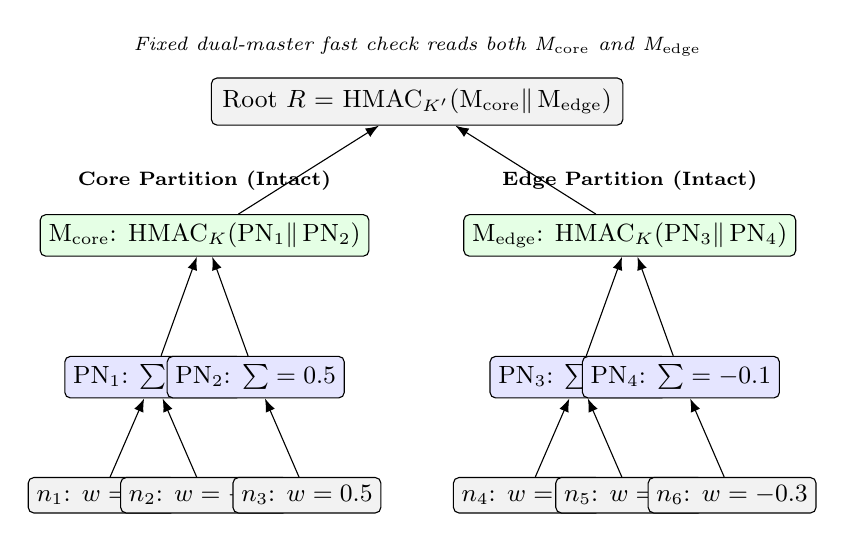
\begin{tikzpicture}[>=Latex, node distance=0.6cm]
  % Styles
  \tikzstyle{neuron}=[draw, rounded corners=2pt, fill=gray!10, inner sep=3pt, font=\small]
  \tikzstyle{pn}=[draw, rounded corners=2pt, fill=blue!10, inner sep=3pt, font=\small]
  \tikzstyle{mn}=[draw, rounded corners=2pt, fill=green!10, inner sep=3pt, font=\small]
  \tikzstyle{root}=[draw, rounded corners=2pt, fill=black!5, inner sep=4pt, font=\small]
  \tikzstyle{lab}=[font=\scriptsize]

  % Left pyramid: Core partition (Intact)
  \node[neuron] (c_n1) at (-4,0) {$n_{1}$: $w=1.2$};
  \node[neuron] (c_n2) at (-2.7,0) {$n_{2}$: $w=-0.7$};
  \node[neuron] (c_n3) at (-1.4,0) {$n_{3}$: $w=0.5$};

  \node[pn] (c_pn1) at (-3.35,1.5) {PN$_1$: $\sum=0.5$};
  \node[pn] (c_pn2) at (-2.05,1.5) {PN$_2$: $\sum=0.5$};

  \draw[->] (c_n1) -- (c_pn1);
  \draw[->] (c_n2) -- (c_pn1);
  \draw[->] (c_n3) -- (c_pn2);

  \node[mn] (c_mn) at (-2.7,3.3) {M$_{\mathrm{core}}$: HMAC$_K$(PN$_1\|\,$PN$_2$)};
  \draw[->] (c_pn1) -- (c_mn);
  \draw[->] (c_pn2) -- (c_mn);

  \node[lab] at (-2.7,4.0) {\textbf{Core Partition (Intact)}};

  % Right pyramid: Edge partition (Intact)
  \node[neuron] (e_n1) at (1.4,0) {$n_{4}$: $w=0.8$};
  \node[neuron] (e_n2) at (2.7,0) {$n_{5}$: $w=0.2$};
  \node[neuron] (e_n3) at (4.0,0) {$n_{6}$: $w=-0.3$};

  \node[pn] (e_pn1) at (2.05,1.5) {PN$_3$: $\sum=1.0$};
  \node[pn] (e_pn2) at (3.35,1.5) {PN$_4$: $\sum=-0.1$};

  \draw[->] (e_n1) -- (e_pn1);
  \draw[->] (e_n2) -- (e_pn1);
  \draw[->] (e_n3) -- (e_pn2);

  \node[mn] (e_mn) at (2.7,3.3) {M$_{\mathrm{edge}}$: HMAC$_K$(PN$_3\|\,$PN$_4$)};
  \draw[->] (e_pn1) -- (e_mn);
  \draw[->] (e_pn2) -- (e_mn);

  \node[root] (root) at (0,5.0) {Root $R$ = HMAC$_{K'}$(M$_{\mathrm{core}}\|\,$M$_{\mathrm{edge}}$)};
  \draw[->] (c_mn) -- (root);
  \draw[->] (e_mn) -- (root);

  \node[lab] at (2.7,4.0) {\textbf{Edge Partition (Intact)}};

  \node[lab] at (0,5.7) {\emph{Fixed dual-master fast check reads both M$_{\mathrm{core}}$ and M$_{\mathrm{edge}}$}};
\end{tikzpicture}
\caption{Hierarchical integrity flow with neurons at the bottom (intact model). Example values illustrate PN sums; masters store HMACs over their PN sets; the root is an HMAC over masters.}
\label{fig:intact_pyramid}
\end{figure}

% Tampered pyramid
\begin{figure}[!htbp]
\centering
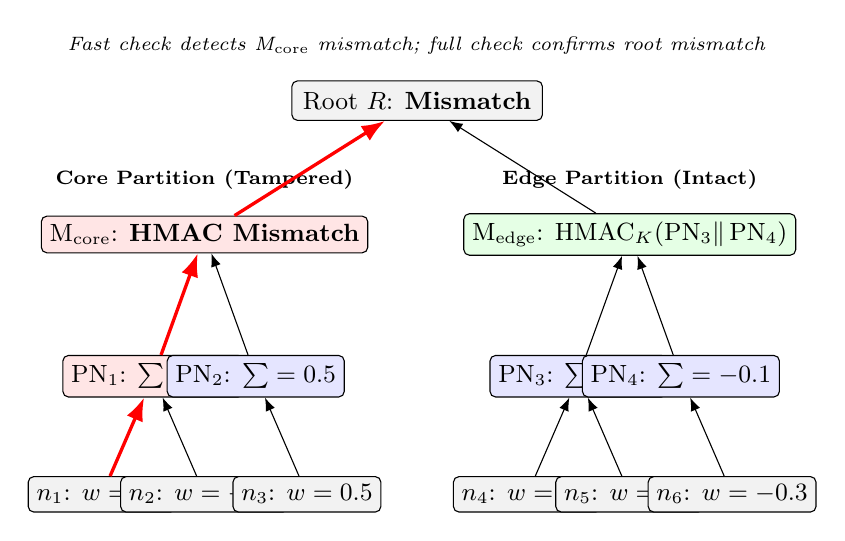
\begin{tikzpicture}[>=Latex, node distance=0.6cm]
  % Styles
  \tikzstyle{neuron}=[draw, rounded corners=2pt, fill=gray!10, inner sep=3pt, font=\small]
  \tikzstyle{pn}=[draw, rounded corners=2pt, fill=blue!10, inner sep=3pt, font=\small]
  \tikzstyle{pnred}=[draw, rounded corners=2pt, fill=red!10, inner sep=3pt, font=\small]
  \tikzstyle{mn}=[draw, rounded corners=2pt, fill=green!10, inner sep=3pt, font=\small]
  \tikzstyle{mnred}=[draw, rounded corners=2pt, fill=red!10, inner sep=3pt, font=\small]
  \tikzstyle{root}=[draw, rounded corners=2pt, fill=black!5, inner sep=4pt, font=\small]
  \tikzstyle{lab}=[font=\scriptsize]

  % Left pyramid: Core partition (Tampered)
  \node[neuron] (c_n1) at (-4,0) {$n_{1}$: $w=1.3$}; % changed from 1.2 to 1.3
  \node[neuron] (c_n2) at (-2.7,0) {$n_{2}$: $w=-0.7$};
  \node[neuron] (c_n3) at (-1.4,0) {$n_{3}$: $w=0.5$};

  \node[pnred] (c_pn1) at (-3.35,1.5) {PN$_1$: $\sum=\mathbf{0.6}$};
  \node[pn]    (c_pn2) at (-2.05,1.5) {PN$_2$: $\sum=0.5$};

  \draw[->,red,very thick] (c_n1) -- (c_pn1);
  \draw[->] (c_n2) -- (c_pn1);
  \draw[->] (c_n3) -- (c_pn2);

  \node[mnred] (c_mn) at (-2.7,3.3) {M$_{\mathrm{core}}$: \textbf{HMAC Mismatch}};
  \draw[->,red,very thick] (c_pn1) -- (c_mn);
  \draw[->] (c_pn2) -- (c_mn);

  \node[lab] at (-2.7,4.0) {\textbf{Core Partition (Tampered)}};

  % Right pyramid: Edge partition (Intact)
  \node[neuron] (e_n1) at (1.4,0) {$n_{4}$: $w=0.8$};
  \node[neuron] (e_n2) at (2.7,0) {$n_{5}$: $w=0.2$};
  \node[neuron] (e_n3) at (4.0,0) {$n_{6}$: $w=-0.3$};

  \node[pn] (e_pn1) at (2.05,1.5) {PN$_3$: $\sum=1.0$};
  \node[pn] (e_pn2) at (3.35,1.5) {PN$_4$: $\sum=-0.1$};

  \draw[->] (e_n1) -- (e_pn1);
  \draw[->] (e_n2) -- (e_pn1);
  \draw[->] (e_n3) -- (e_pn2);

  \node[mn] (e_mn) at (2.7,3.3) {M$_{\mathrm{edge}}$: HMAC$_K$(PN$_3\|\,$PN$_4$)};
  \draw[->] (e_pn1) -- (e_mn);
  \draw[->] (e_pn2) -- (e_mn);

  \node[root] (root_bad) at (0,5.0) {Root $R$: \textbf{Mismatch}};
  \draw[->,red,very thick] (c_mn) -- (root_bad);
  \draw[->] (e_mn) -- (root_bad);

  \node[lab] at (2.7,4.0) {\textbf{Edge Partition (Intact)}};

  \node[lab] at (0,5.7) {\emph{Fast check detects M$_{\mathrm{core}}$ mismatch; full check confirms root mismatch}};
\end{tikzpicture}
\caption{Tamper propagation with neurons at the bottom. A small weight change in $n_1$ shifts PN$_1$'s sum, which flips M$_{\mathrm{core}}$'s HMAC; the root digest then mismatches. Red highlights show the bubble-up path.}
\label{fig:tampered_pyramid}
\end{figure}

% Horizontal pipeline (PNG)
\begin{figure}[!htbp]
\centering
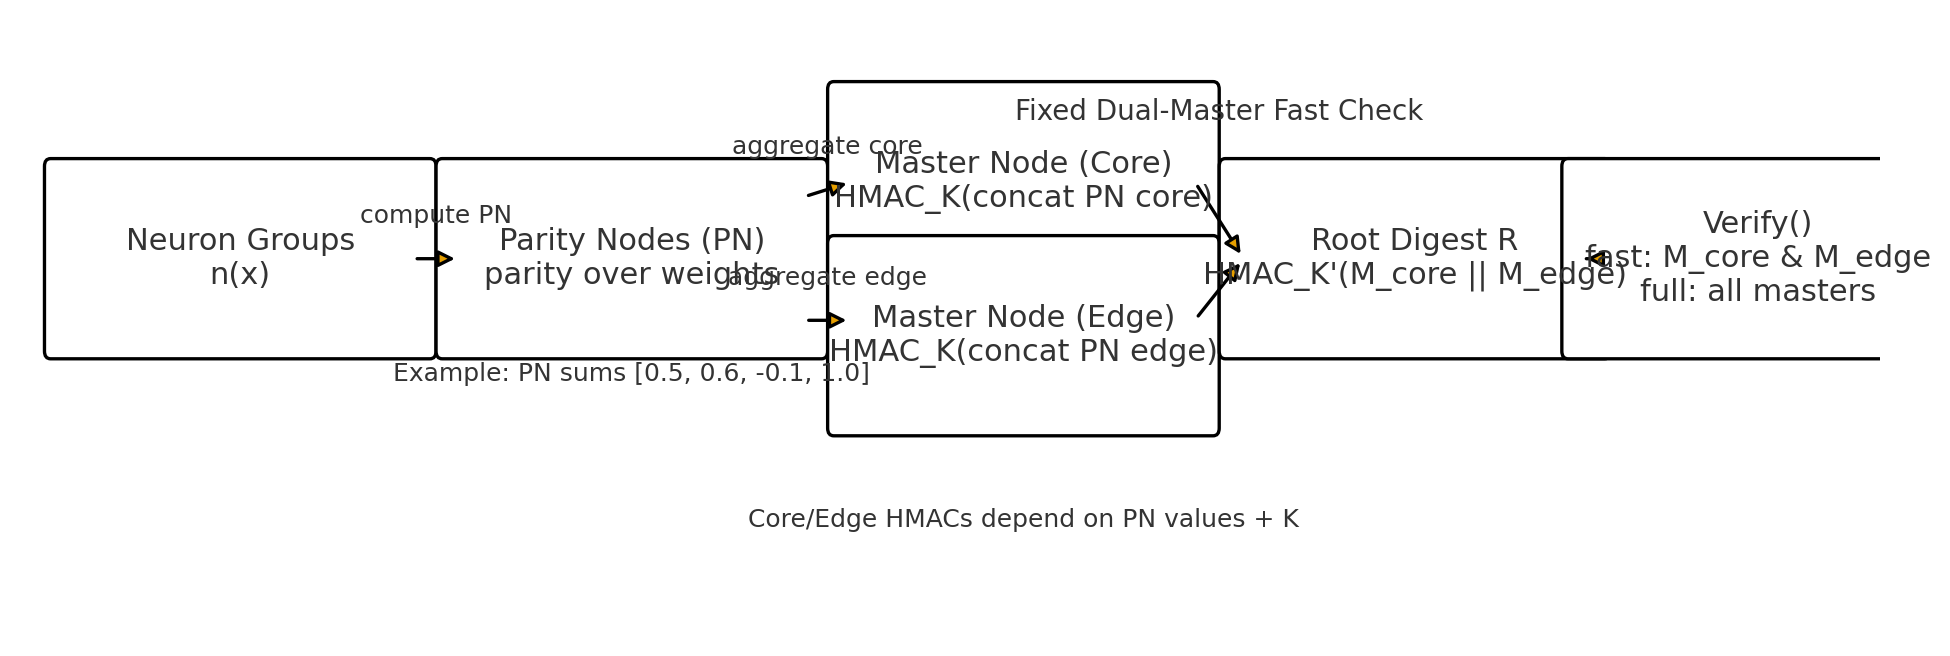
\includegraphics[width=\linewidth]{pnm_pipeline.png}
\caption{Horizontal verification pipeline: neuron groups $\rightarrow$ parity nodes $\rightarrow$ fixed masters (core/edge) $\rightarrow$ root digest $\rightarrow$ Verify(). Fast checks read the two fixed masters each inference; full checks verify all masters periodically.}
\label{fig:pipeline}
\end{figure}

\FloatBarrier
\section{Conclusion}
Hardened PNM anchors model integrity in an HMAC-rooted chain-of-trust and augments structural checks with semantic canaries. The design resisted all tested attacks in simulation with negligible overhead, offering a practical path to verifiable AI integrity in production.

\paragraph{Availability}
Reference implementation and scripts: \href{https://github.com/stevejhorton/PNM}{\texttt{github.com/stevejhorton/PNM}}.

\clearpage
\bibliographystyle{plain}
\bibliography{references}

\appendix
\section{Appendix: Verifier Sketch}
\begin{algorithm}[H]
\caption{Fixed dual-stage verification with canaries}
\begin{algorithmic}[1]
\State Load locked parity map, master HMACs, root digest
\State \textbf{Fast check}: recompute two fixed masters $(m_{\mathrm{core}}, m_{\mathrm{edge}})$; verify HMACs
\If{fail} \State \Return Alarm \EndIf
\State \textbf{Full check}: recompute all masters; verify root digest
\If{fail} \State \Return Alarm \EndIf
\State \textbf{Canaries}: evaluate $\{x_c\}$ and compare to $\{y_c^\star\}$
\If{any fail} \State \Return Alarm \Else \Return Verified \EndIf
\end{algorithmic}
\end{algorithm}

\end{document}
